\label{sec:hitbox}
Hitboxen sind Approximationen für Modelle in einer Simulation. Sie ersetzen das konkrete Modell dabei für Kollisionen gegenüber der Kollisionserkennung komplett.\\
Der Term Hitbox suggeriert die verwendung einer Box/eines Quaders zur Approximation. Das ist historisch bedingt. Der Term ist allerdings auch für andere Approximationsformen etabliert.\\
Die Diskrepanz zwischen Hitbox und Model wirkt sich negativ auf den physikalischen Realismus aus. Trotzdem wird von Entwicklern so viel wie kontextuell vertretbar approximiert, um Rechenzeit zu sparen und Echtzeitanforderungen zu genügen.

\begin{figure*}
	\begin{subfigure}[t]{0.45\textwidth}
		\centering
		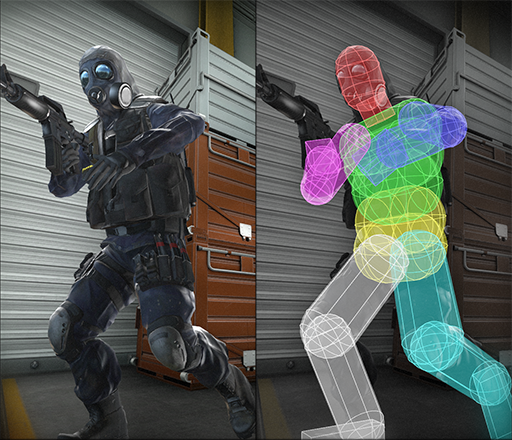
\includegraphics[width=1\textwidth]{./res/csgo_hitbox.png}
		\caption{Hitbox des Spieler-Modells aus dem Videospiel Counter Strike: Global Offensive; sichtbares Modell(links), mit eingeblendeter Hitbox (rechts)}
%%TODO source for pic
		\label{fig:chitbox}
	\end{subfigure}
~
	\begin{subfigure}[t]{0.2\textwidth}
		\centering
		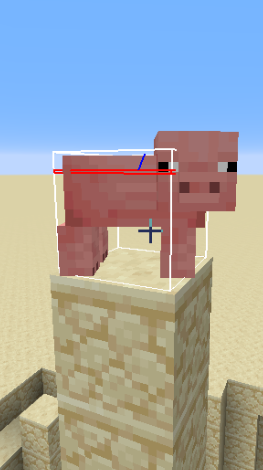
\includegraphics[width=1\textwidth]{./res/pig_hitbox.png}
		\caption{Hitbox eines NPC-Modells (Schwein) aus dem Videospiel Minecraft; Hitbox in weiß}
		\label{fig:mphitbox}
	\end{subfigure}
~
	\begin{subfigure}[t]{0.2\textwidth}
		\centering
		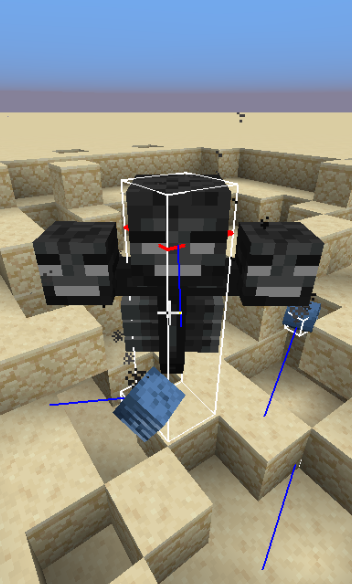
\includegraphics[width=1\textwidth]{./res/wither_hitbox.png}
		\caption{Hitbox eines NPC-Modells (Wither) aus dem Videospiel Minecraft; Hitbox in weiß}
		\label{fig:mwhitbox}
	\end{subfigure}

	\caption{Güten von Hitboxen}
	\label{fig:hitbox}
\end{figure*}

Die Abbildungen~\ref{fig:hitbox} zeigen Hitboxen in 2 verschiedenen Spielen.\\
\ref{fig:chitbox} zeigt das Spielermodell aus dem Spiel Counter-Strike: Global Offensive (CSGO). Links ist dabei das sichtbare Modell zu sehen, während rechts die Hitboxen eingeblendet sind. Die Hitboxen, welche hier nichmal mehr Boxen sind, sondern Ellipsoiden, decken das sichtbare Modell relativ genau ab. Ebenfalls zu erkennen ist die Partition in einzelne Hitboxen, zu sehen an den verschiedenen Farben der Hitboxen im rechten Bild.\\
Einzelne Details des Spielermodells, wie Riemen und Taschen an der Ausrüsung, sind nicht essentiell und werden daher auch physikalisch nicht abgebildet.\\
\ref{fig:mphitbox} und \ref{fig:mwhitbox} zeigen Hitboxen aus dem Spiel Minecraft bei zwei NPCs (Non-Player-Character (zu Deutsch: Nicht-Spieler-Charakter)). Es ist dort klar zu erkennen, dass die Hitboxen nicht sehr genau mit dem sichtbaren Modell übereinstimmen. Mehr noch: Die Minecraft-Hitboxen sind Koordinatenachsenparallel, d.h. Kanten verlaufen immer entlang der Koordinatenachsen der Raumrepräsentation.\\
Es wird versucht die Unterschiede zu rechtfertigen:\\
CSGO ist ein Shooter. Schnelle Reaktion und genaues Zielen sind ein hauptbestandteil des Produkts. Zudem ist CSGO ein hochkompetitiver E-Sport, der professionell gespielt wird. Es geht dabei um Preisgelder im siebenstelligen Bereich \cite{csgoprice}. Akkurate und, aus der perspektive des Spielers deterministische Hitboxen sind daher essenziell für das Produkt.\\
Die Partition der Hitboxen in CSGO ergibt sich direkt aus einer Anforderung der Anwendung, Schusstreffer auf verschiedene Teile des Spielermodells unterschiedlich zu bewerten. Beispielsweise verursacht der Treffer am Kopf am meisten Schaden. CSGO modelliert die unterschiedlichen Treffbaren teile des Modells also über mehrere Hitboxen.\\
Minecraft ist ein Sandbox Aufbauspiel. Ziel des Spiels ist der Bau von beliebigen Gebäuden, Tunneln, die Kreation von Maschinen oder das Erkunden von Gebieten.\\
In Minecraft steckt auch eine erhebliche Summe Geld. Am 15. September 2014 kaufte Microsoft die Entwicklerfirma und die rechte am Spiel für ca. 2,5 Milliarden Dollar \cite{buyminecraft}.\\
Das Kampfsystem in Minecraft forciert keine schnellen und genauen Treffer auf Gegner. Die gesamte Spielwelt ist aus sichtbaren Achsenparallel aufgestellten Würfeln gegeben, sind also Deckungsgleich mit entsprechenden achsenparallelen Hitboxen. Minecraft macht es sich einfach, da keine konkreten Anforderungen hinsichtlich Genauigkeit bestehen. Tatsächlich wird eine künstlich kleinere Hitbox manchmal sogar eingesetzt um einen Treffer zu erschweren (vgl. Abbildung \ref{fig::mwhitbox}).\\

